% F092｜derive 原创简明教学示意图
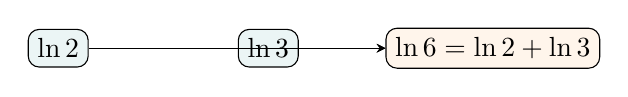
\begin{tikzpicture}[>=stealth,scale=.92]
\node[draw,rounded corners,fill=teal!8] (a) at (0,0){$\ln2$};
\node[draw,rounded corners,fill=teal!8] (b) at (2.9,0){$\ln3$};
\node[draw,rounded corners,fill=orange!8] (c) at (6,0){$\ln6=\ln2+\ln3$};
\draw[->] (a)--(c);\draw[->] (b)--(c);
\end{tikzpicture}
